\documentclass[12pt,twoside]{article}

% packages
\usepackage{amssymb,amsmath,amsbsy}
\usepackage{graphicx}
\usepackage[includeheadfoot, top=1in, bottom=1in, hmargin=1in]{geometry}
\usepackage{fancyhdr}
\usepackage{verbatim}
\usepackage{url}
\usepackage{enumitem}
\usepackage{multicol}

% commands
\newcommand{\given}{\,|\,}
\newcommand{\dd}{\mathrm{d}}
\newcommand{\msun}{\mathrm{M}_\odot}
\newcommand{\projectname}[1]{\begin{center} {\huge {#1}} \end{center}}
\newcommand{\kms}{\mathrm{km}~\mathrm{s}^{-1}}

% environments
\newcommand{\problemname}{Problem}
\newcounter{problem}
\newenvironment{problem}{\paragraph{\problemname~\theproblem:}\refstepcounter{problem}}{}
 
\pagestyle{fancy}

\lhead{Due: 10/27/14}
\chead{}
\rhead{}
\lfoot{Galactic Dynamics}
\cfoot{\thepage}
\rfoot{Fall 2014}

\begin{document}

\projectname{Project 2}

The goal of this problem set is to investigate the orbits of disk stars near the Sun. 

\begin{problem} 
{\bf Write a Leapfrog integrator in Python.} There is a description of the Leapfrog algorithm in Binney and Tremaine, as well as in Numerical Recipes.  Write your Leapfrog class or function in such a way that you can specify (as arguments to your integrator) a function that computes the accelerations, a set of initial conditions, a timestep, and a number of steps, and have it return the orbit. By doing this, we keep the code general so we can swap in different acceleration fields or initial conditions without changing huge sections of the core code. Below is a skeleton of how you might do this, and an example of passing in a specific acceleration function.

\begin{verbatim}
def leapfrog_integrate(acceleration_func, args=(), x0, v0, dt, nsteps):
    # the `args' keyword will let you specify additional arguments or
    #	parameters that the acceleration function might need. For
    #	example, the mass in the point-mass potential, which you 
    #	might want to change
    func = lambda x: acceleration_func(x, *args)
    
    # ... implement leapfrog scheme, but use func() to evaluate the 
    #     acceleration instead of acceleration_func()

def point_mass_acceleration(x, m):
    """ Compute the acceleration due to a point mass 
        at the origin with mass m 
    """
    acc = -G*m*x / np.linalg.norm(x,axis=0)**3
    return acc
    
m = 1.
orbit = leapfrog_integrate(point_mass_acceleration, args=(m,),
				                           x0=np.array([1.,0.]), v0=np.array([6.2,0.]),
				                           dt=0.2, nsteps=1000)
\end{verbatim}

\noindent\hfil\rule{0.5\textwidth}{.4pt}\hfil

\vspace{2em}

Test your integrator on the simple harmonic oscillator (SHO) potential,
\begin{equation}
	\Phi(x) = \frac{1}{2}\omega^2 x^2
\end{equation}
where $\omega$ is a free parameter. {\bf Integrate an orbit in this potential with}
\begin{align}
	\omega &= 2.\\
	x_0 &= 1.\\
	v_0 &= 0.
\end{align}
{\bf and verify that your orbit looks like the plot in Figure~\ref{fig:sho}}.

\begin{figure*}[!h]
\begin{center}
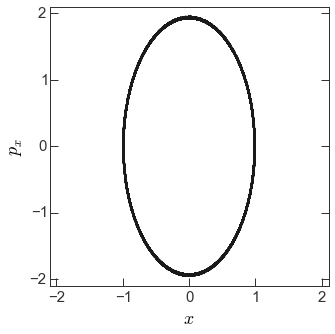
\includegraphics[width=0.5\textwidth]{sho.png}
\caption{ Example of an orbit in the SHO potential with $\omega=2$. }\label{fig:sho}
\end{center}
\end{figure*}

\end{problem}

\begin{problem}
{\bf Choose an analytic form for the potential of the disk of the Milky Way.} There are many options for thin, disk-like potentials (see Binney and Tremaine). The exact form you use doesn't matter, but {\bf explain your choice.} In the next problems, we will use the potential to integrate orbits from observed stars. To do this, we will need to choose parameters for the potential that are somewhat realistic. {\bf Find the parameters of the potential by fitting the value of the rotation curve at the Sun's position to your favorite observational constraint on this value. You can do this by eye, but plot the rotation curve of your potential along the disk midplane for several different radii. What is unrealistic about your rotation curve?} Again, it doesn't matter what value you use, but {\bf explain your choice. }

\end{problem}

\begin{problem}
Using the new Hipparcos data file --- the new file is exactly the same as that from the previous project, but now has a column for radial velocities and uncertainties in the radial velocities --- read in the data and apply some simple quality cuts. We will, again, reject large fractional parallax uncertainties, binary stars, and now reject large fractional proper motion uncertainties. Only include data for which:
\begin{align}
 \pi &> 0\\
\sigma_\pi / \pi &< 0.05\\
\sigma_{\mu_l} / \mu_l &< 0.05\\
\sigma_{\mu_b} / \mu_b &< 0.05
\end{align}
where $\pi$ is the parallax, and $(\mu_l,\mu_b)$ are the proper motions in Galactic coordinates. Only some of the stars have measured radial velocities, so you'll also want to make a cut to remove any star with a radial velocity that is NaN. You should be left with 3880 stars. {\bf Convert the positions and velocities of these stars to cartesian coordinates in a Galactocentric reference frame.} To do this, you need to assume something about the velocity of the Sun relative to the local standard of rest (LSR). We will all use the same LSR velocity of:
\begin{align}
U &= 11.1~\kms\\
V &= 12.24~\kms\\
W &= 7.25~\kms
\end{align}
from Sch\"onrich \& Binney (2010). You will also need to use the value of the circular velocity at the Sun that you used for the previous problem. You may use \texttt{astropy.coordinates} to help you with this conversion, but the full transformation is not built in to the package so you will have to write some of the code yourself. To check that you've done the conversion properly, {\bf make plots of the positions and velocities of all stars.} For example, $x$ vs. $y$, and $v_x$ vs. $v_y$. Your plots should look like those in Figures~\ref{fig:xyz}-\ref{fig:vxyz}.

{\bf What is interesting about the density of points in these plots? What does this imply?}

\end{problem}

\begin{problem}
Once you have cartesian positions and velocities for all of these stars, {\bf integrate the orbits of the stars for 2 Gyr in the disk potential you chose from Problem 2.} (Hopefully you wrote your integration function in such a way that you may integrate many orbits in parallel with numpy arrays...) {\bf Plot a few orbits in the meridional plane (cylindrical $R$ vs. $z$). Explain (qualitatively) the properties of the orbits.}

Now we will get more quantitative. {\bf For each orbit, compute the pericentric and apocentric distances, the orbital periods in the radial, azimuthal, and vertical directions, and the maximum height, $|z|$, above or below the midplane. Make histograms of each of these quantities individually, then create a scatter plot matrix by plotting each quantity vs. every other quantity in a big grid of plots.} You may use the \texttt{pandas} package, which has a convenient function for generating such plots (\texttt{pandas.plotting.scatter\_matrix}).

{\bf Explain in a paragraph or two what interesting features you see in these data. What quantities are correlated? Which quantities show no correlations? Do any of these observations surprise you? How would these features change if we looked at a larger volume of stars, say, within 1~kpc of the Sun instead of within 100 pc?}

\end{problem}

\begin{figure*}[!h]
\begin{center}
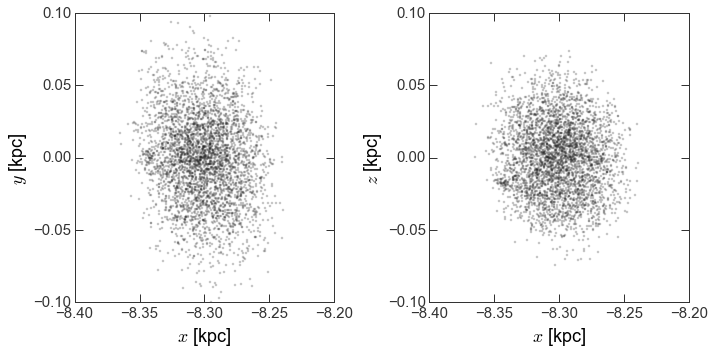
\includegraphics[width=0.7\textwidth]{xyz.png}
\caption{ Positions of selected Hipparcos stars in Galactocentric, cartesian coordinates. }\label{fig:xyz}
\end{center}
\end{figure*}

\begin{figure*}[!h]
\begin{center}
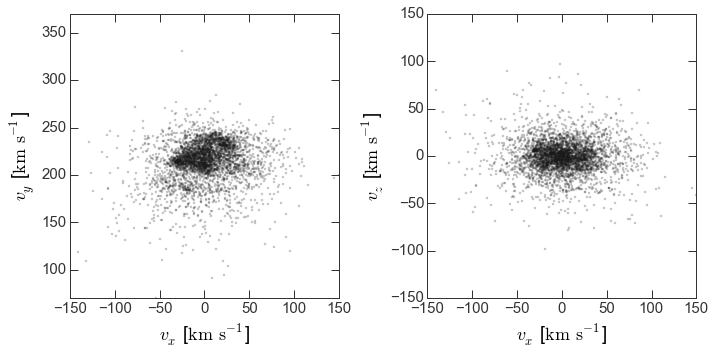
\includegraphics[width=0.7\textwidth]{vxyz.png}
\caption{ Velocities of selected Hipparcos stars in Galactocentric, cartesian coordinates. }\label{fig:vxyz}
\end{center}
\end{figure*}

\end{document}

%\begin{figure*}[!h]
%\begin{center}
%\includegraphics[width=\textwidth]{PATH}
%\caption{ CAPTION }\label{fig:FIGNAME}
%\end{center}
%\end{figure*}